\section{Ausgangslage}\label{chapter:Ausgangslage}

Die Ausgangslage dieser Arbeit ist durch eine fehlende einheitliche digitale Dokumentenablage geprägt. Dokumente werden in unterschiedlichen Strukturen gespeichert, sind nur mit hohem Aufwand auffindbar und unterliegen keiner durchgängig zentral verwalteten Zugriffskontrolle. Dadurch entstehen organisatorische und technische Probleme, die sowohl die tägliche Arbeit als auch die Sicherheit und Nachvollziehbarkeit der Dokumentenverwaltung beeinträchtigen.

\begin{figure}[htbp]
    \centering
    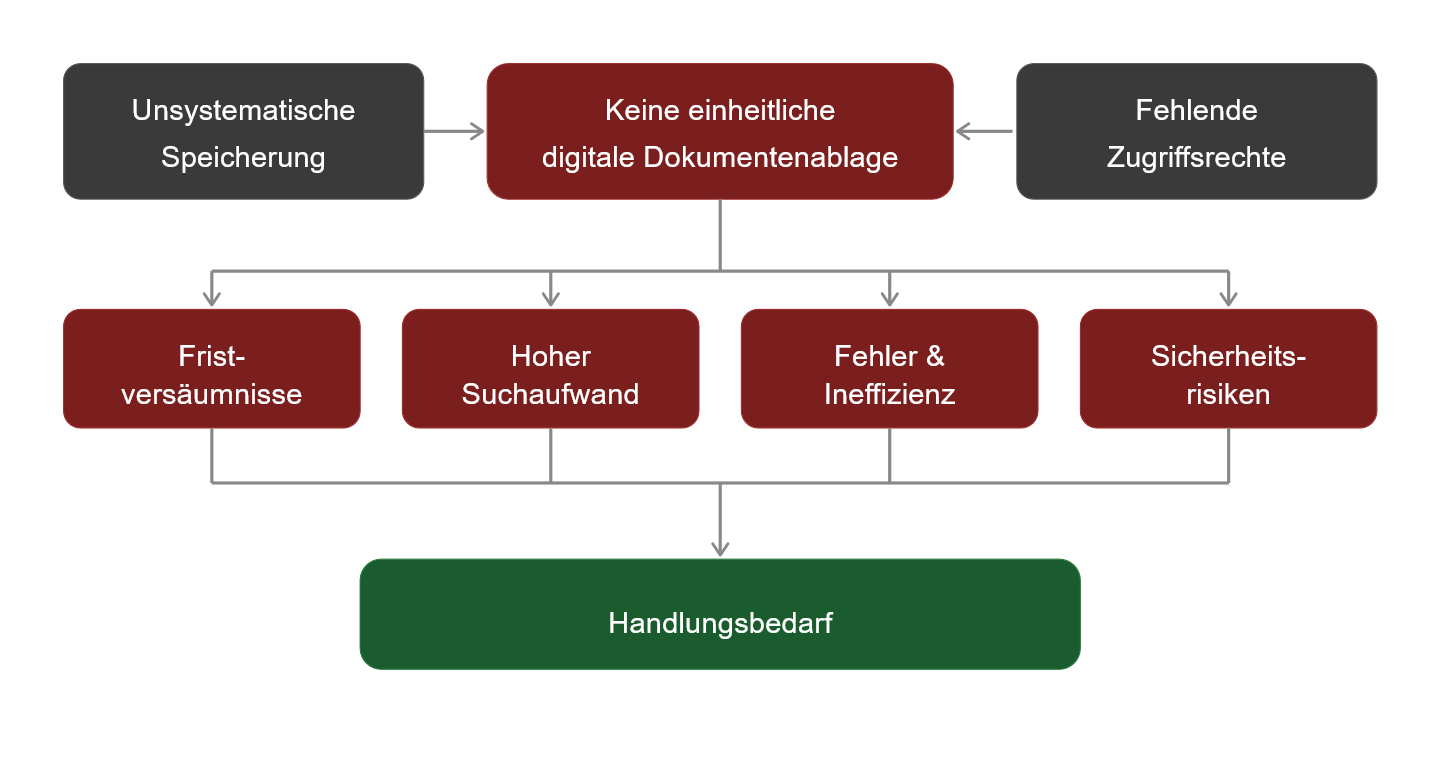
\includegraphics[width=0.95\textwidth]{content/img/4_deployment/ausgangslage.png}
    \caption{Schematische Darstellung der Ausgangslage}
    \label{fig:ausgangslage}
\end{figure}

Abbildung \ref{fig:ausgangslage} zeigt diese Situation in vereinfachter Form. Eine unsystematische Speicherung von Dokumenten und fehlende Zugriffsrechte führen dazu, dass keine einheitliche digitale Dokumentenablage vorhanden ist. Daraus ergeben sich in der Praxis ein hoher Suchaufwand, Fristversäumnisse, Fehler und Ineffizienz in Arbeitsabläufen sowie erhöhte Sicherheitsrisiken. Insgesamt entsteht daraus ein klarer Handlungsbedarf, die Dokumentenverwaltung strukturiert, sicher und effizient neu zu gestalten.